\section{Metodologia}


\begin{frame}

    \frametitle{Metodologia}

   \begin{figure}[!htbp]
   	\centering
   	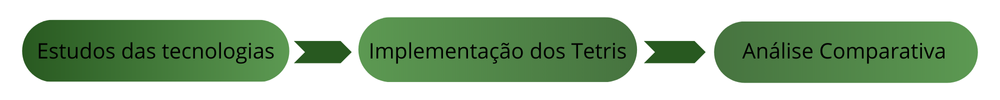
\includegraphics[scale=0.55]{imagens/Metodologia.png}
   	%\\\small{\textbf{Fonte:} Elaborada pelo autor (fonte é opcional)}%
   \end{figure}
\end{frame}

\begin{frame}
	
	\frametitle{Metodologia: Tetris}
	
	\begin{columns}[t]
		
		\begin{column}{7cm}
			
			Tetris é um jogo de quebra-cabeça, onde em uma grade de 10 colunas e 20 linhas, o jogador empilha formas geometricas denominadas tetrominós,
			assim que uma linha inteira é preenchida, essa linha é retirada e as outras serão deslocadas para baixo, assim liberando espaço para a continuidade do jogo
			
		\end{column}
		
		\begin{column}{7cm}
			
			\begin{figure}[!htbp]
				\centering
				\caption{Os 7 tetraminós}
				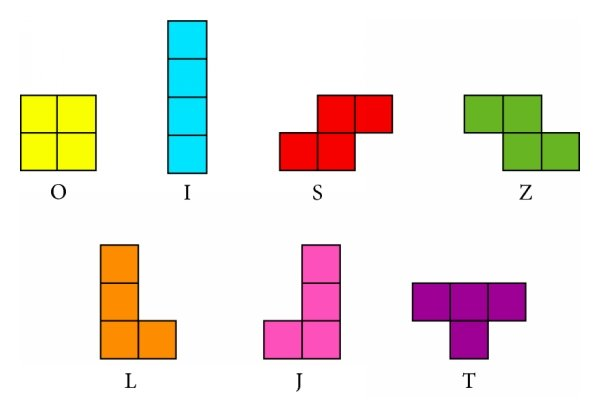
\includegraphics[scale=1.2]{imagens/tetraminoes.png}
				%\\\small{\textbf{Fonte:} Elaborada pelo autor (fonte é opcional)}%
			\end{figure}
			
		\end{column}
		
	\end{columns}
\end{frame}
